\documentclass[12pt]{article}

% Packages
\usepackage[utf8]{inputenc}
\usepackage[T1]{fontenc}
\usepackage{amsmath}
\usepackage{amsfonts}
\usepackage{amssymb}
\usepackage{graphicx}
\usepackage{geometry}
\usepackage{float}
\usepackage{caption}
\usepackage{hyperref}
\usepackage{cite}
\usepackage{xcolor}
\usepackage{booktabs}
\usepackage{enumitem}

% Page setup
\geometry{
    letterpaper,
    margin=0.75in,
    top=0.75in,
    bottom=0.75in
}

% Hyperlink setup
\hypersetup{
    colorlinks=true,
    linkcolor=blue,
    filecolor=magenta,      
    urlcolor=cyan,
    citecolor=red
}

% Title page information
\title{\textbf{MEMORANDUM}}
\author{}
\date{\today}

\begin{document}

% Title page
\maketitle

\vspace{-1cm}
\begin{center}
\textbf{TO:} Dr. Arthur Erdman \\
\textbf{FROM:} Peyton Lettau, Sebastian Hondl, John Robinson, Will McConnell \\
\textbf{SUBJECT:} Progress Report 1 - Miniature Tabletop Greenhouse Mechanism Design \\
\textbf{DATE:} \today
\end{center}

\vspace{0.5cm}

\section*{EXECUTIVE SUMMARY}

This memorandum summarizes the progress on the miniature tabletop greenhouse mechanism design project. Through systematic type synthesis and patent analysis, we have identified the Watt I six-bar mechanism as the optimal topology for path generation. The work demonstrates the inadequacy of four-bar solutions for the given constraints and establishes a clear path forward for dimensional synthesis and prototype development.

\section*{PROBLEM STATEMENT}

The project addresses the challenge of designing a mechanism for a miniature tabletop greenhouse that can simultaneously open both top and front panels while meeting strict spatial constraints. A greenhouse creates a controlled microclimate by admitting short-wave solar radiation while slowing heat loss, raising temperature and humidity to support plant growth. In miniature formats, these same principles are compressed to a smaller area, but certain criteria become more difficult to maintain due to scaling effects.

\subsection*{Design Requirements}
Key requirements include:

\begin{itemize}
    \item Single-degree-of-freedom motion with one user input
    \item Compact tabletop dimensions (18" × 18" × 24")
    \item Support for 5 lb panels with smooth motion
    \item Mechanism must not extend beyond greenhouse silhouette when closed
    \item Enable access to plants from both top and front faces simultaneously
    \item The opening above the enclosure must be >90\% of the depth of the enclosure
    \item Allow front and top of the enclosure to be positioned at any position between open and close and remain in place
    \item Fold the top and front panels above the enclosure, creating unobstructed access for plant maintenance
\end{itemize}

A figure of the coupler point analysis for mechanism path generation is shown below. The pink zones are areas the coupler, assumed to be at the end of the front panel, cannot be in to satisfy the criteria. The path is only for demostration and is not a final solution.

\begin{figure}[H]
    \centering
    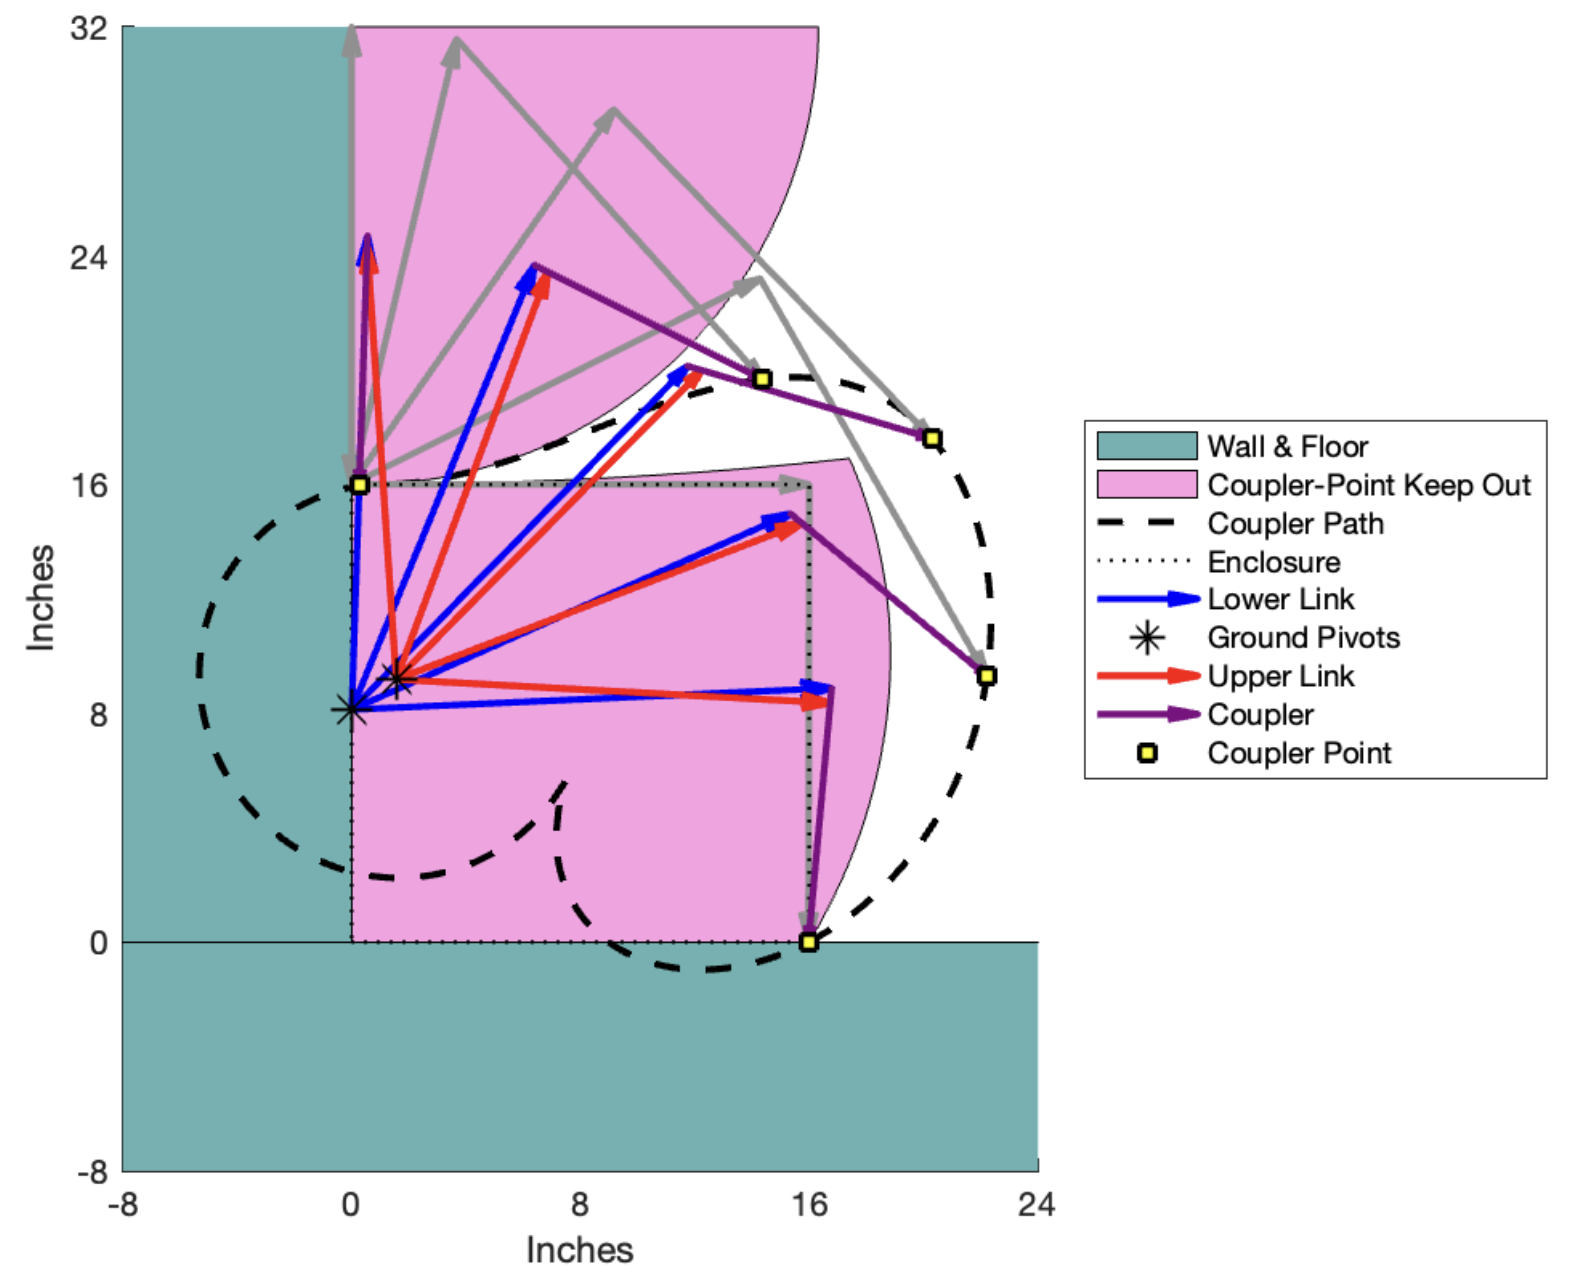
\includegraphics[width=0.7\textwidth]{../03_Images/Coupler Points.png}
    \caption{Coupler point analysis for mechanism path generation.}
    \label{fig:coupler_points}
\end{figure}

\section*{PATENT ANALYSIS}

Analysis of existing solutions revealed significant scaling challenges. Common access solutions range from simple to engineered approaches. Low-tech options include cloches and cold-frame-style hinged lids, sliding or lift-off clear panels, roll-up soft sides, zipper covers, and magnetic or hook-and-loop closures. More refined mechanisms add hold-open features and controllable venting: front-hinged or top-hinged lids with friction hinges or gas springs; scissor-link or four-bar "pop-top" lids that lift and translate to clear the aperture; rack-and-pinion or cam-assisted lift for precise positioning; and side-access tambour doors for tight spaces.

\subsection*{Detailed Patent Analysis}

\textbf{Patent 1 - Portable Greenhouse (Koziol, 1974 \cite{Koziol1974}):} This patent represents a practical full-scale greenhouse solution using a different opening and closing system. While effective at full size, scaling this design down presents significant operational challenges. The plurality of covered sides becomes more complex to operate when the greenhouse is positioned on a desk, and the mechanism components become proportionally smaller and more difficult to manipulate.

\textbf{Patent 2 - Full-Scale Greenhouse Covering (Jaderloon Company, 1999 \cite{Jaderloon1999}):} This design functions to keep out rainwater using cable systems, rotating shafts, and tension drums that require very precise alignment. While effective at full scale, these systems are not feasible for small-scale applications. Scaling down would make parts more fragile, expensive, and difficult to assemble. Additionally, the tension in cables does not scale proportionally when reduced to smaller sizes, leading to inadequate performance or excessive complexity.

\textbf{Patent 3 - Greenhouse Window Mechanism (Bom, 1978 \cite{Bom1978}):} This patent shows an opening and closing mechanism for greenhouse windows that demonstrates potential scalability to the current project. The mechanism relies on rigid bars and rotational joints, making it more suitable for adaptation to small-scale applications. The triangular guide-bar linkage coordinates multiple vents with stable geometry, offering promise for synchronized, multi-panel tabletop access.

\section*{DESIGN PROCESS}
\subsection*{Solution Approach Options}
The design problem can be formulated through multiple approaches:

\begin{enumerate}
    \item \textbf{Path Generation}: A point on the front panel is selected as the coupler point, and a linkage is synthesized to guide this point through a series of precision positions while maintaining the front panel attachment through a pivot connection.
    
    \item \textbf{Motion Synthesis}: The top and front panels are linked within the mechanism, and the mechanism is synthesized based on the angular and positional relationships of the front panel throughout its range of motion.
\end{enumerate}

\subsection*{Selected Solution Approach}
For this project, the path generation approach was selected as the primary design methodology. Initial work attempted to synthesize a four-bar linkage for this task, but analysis indicates that a satisfactory four-bar solution is unlikely to exist within the given constraints. However, it appears probable that an effective solution can be achieved using linkages with additional degrees of freedom, such as six-bar or eight-bar mechanisms.

\section*{TECHNICAL APPROACH}

\subsection*{Type Synthesis Process}

Following Erdman and Sandor (1990) methodology \cite{Erdman1990}, we applied Gruebler's equation $F = 3(n-1) - 2f_1 - f_2$ for planar mechanisms. Initial four-bar analysis ($n=4$, $f_1=4$) revealed no feasible solutions within spatial constraints. This necessitated exploration of six-bar mechanisms ($n=6$, $f_1=7$).

\subsubsection*{Four-Bar Analysis}
Initial synthesis attempts demonstrated that four-bar linkages cannot simultaneously satisfy the spatial constraints—ground pivots must be located at the base within 8 cm height with maximum 25 cm separation—and achieve the required door motion with translation through three precision positions. The compact greenhouse envelope combined with ground pivot placement restrictions resulted in no feasible four-bar solutions.

\subsubsection*{Six-Bar Mechanism Development}
Using the equation $n-(F+3)=T+2Q+3P$ for link types, where $T$, $Q$, and $P$ represent ternary, quaternary, and pentagonal links respectively, we find that $6-(1+3)=2$ for our six-bar, single-DOF mechanism. The standard kinematic link set solution (KLSS) comprises 2 ternary links and 4 binary links, providing the foundation for mechanism topology development.

Systematic enumeration of basic kinematic chains (BKCs) from this KLSS, with application of the degree-of-freedom distribution criterion to eliminate configurations containing zero-freedom subchains, yields two valid BKCs: the Watt chain, characterized by two ternary links sharing a common connection, and the Stephenson chain, where the ternary links are separated by binary links.

\begin{figure}[H]
    \centering
    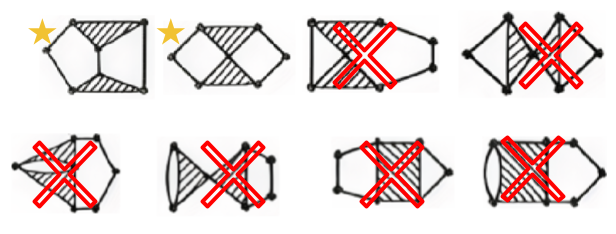
\includegraphics[width=0.7\textwidth]{../03_Images/6 Bar options.png}
    \caption{Six-bar mechanism topology options}
    \label{fig:six_bar_options}
\end{figure}

\subsection*{Topology Selection}

Five topological variations were evaluated: Watt I, Watt II, Stephenson I, Stephenson II, and Stephenson III. The critical differentiator was ground pivot accessibility. Watt II, Stephenson II, and Stephenson III require ternary ground links with three ground pivots, which cannot be accommodated on the compact greenhouse base structure.

\begin{figure}[H]
    \centering
    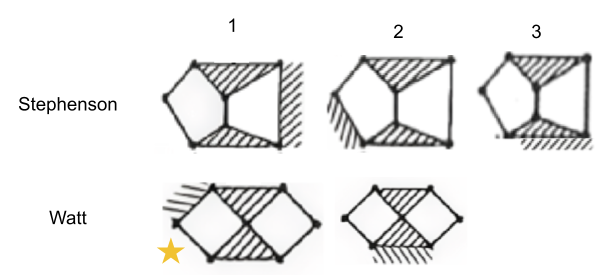
\includegraphics[width=0.7\textwidth]{../03_Images/Stephenson and Watt.png}
    \caption{Stephenson and Watt chain configurations}
    \label{fig:stephenson_watt}
\end{figure}

\section*{SOLUTION SELECTION}

The Watt I configuration emerged as optimal, providing:
\begin{itemize}
    \item Two accessible ground pivots (15-20 cm separation)
    \item Compact dual-loop structure with 8-20 cm link lengths
    \item Favorable transmission angle characteristics
    \item Single-degree-of-freedom motion with one input
\end{itemize}

All seven joints are specified as revolute (pin) joints for manufacturing simplicity. The configuration positions the binary link connected to ground pivot $G_A$ as the input crank, guiding the door panel through three precision positions: closed, ventilation, and fully open.

\section*{RESULTS AND ANALYSIS}

The systematic type synthesis process has successfully identified the Watt I six-bar mechanism as the optimal topology for the greenhouse application. This configuration provides:

\begin{itemize}
    \item Two accessible ground pivots positioned at the front base edge
    \item Compact dual-loop structure with appropriate link lengths
    \item Favorable transmission angle characteristics
    \item Single-degree-of-freedom motion with one input
    \item Spatial compatibility within the greenhouse envelope
\end{itemize}

The selected configuration positions the binary link connected to ground pivot $G_A$ as the input crank, accessible for external user interaction while the mechanism guides the door panel through the three precision positions: closed, ventilation, and fully open.

\section*{FUTURE WORK}

The next phase of the project will focus on:

\begin{itemize}
    \item \textbf{Dimensional synthesis}: Detailed design of the Watt I mechanism with specific link lengths and joint positions
    \item \textbf{Optimization}: Optimization of link lengths and joint positions to achieve optimal performance
\end{itemize}

\section*{CONCLUSION}

The systematic type synthesis process has successfully identified the Watt I six-bar mechanism as the optimal solution for the greenhouse application. This configuration provides the necessary design flexibility while meeting all spatial constraints and performance requirements. The work establishes a clear foundation for dimensional synthesis and prototype development.

\vspace{1cm}

\begin{center}
\textbf{Prepared by:} Project Team \\
\textbf{Date:} \today
\end{center}

% References
\bibliographystyle{ieeetr}
\bibliography{references}

\end{document}
